\documentclass[conference]{IEEEtran}
\usepackage[utf8]{inputenc}
\IEEEoverridecommandlockouts
% The preceding line is only needed to identify funding in the first footnote. If that is unneeded, please comment it out.
\usepackage{cite}
\usepackage{amsmath,amssymb,amsfonts}
\usepackage{algorithmic}
\usepackage{graphicx}
\usepackage{textcomp}
\usepackage{xcolor}
\usepackage{geometry}
\usepackage{float}
\usepackage{adjustbox}
\graphicspath{ {./Images/} }

\usepackage{biblatex} %Imports biblatex package

 
\title{
Analysis of The Performance Deep Learning Algorithms In Video Games\\
\vspace{5mm}
\large Department of Computing \\
\vspace{3mm} 
\large Letterkenny Institute of Technology \\
\vspace{3mm} 
\large Artificial Intelligence 2
}
\author{By Ultan Kearns}
\date{\today}

\begin{document}

\maketitle
\begin{abstract}
    This paper aims to analyze deep learning algorithms and methodologies by utilizing an AI(Artificial Intelligence) Agent to perform specified tasks in simulated environments.  For the purpose of this paper I will be analyzing the Agents performance in video games and will be weighing the pros and cons of each algorithm in respect to the Agent's performance.  Each game has a specific goal for the Agent to complete and the Agent's performance will be evaluated based on certain goals and objectives present in each game discussed in this paper. 
    \\
    \\
    Key Words: AI, Deep Learning, Games
\end{abstract}
\section{Introduction}
\subsection{Purpose of Paper}
The purpose of this paper is to compare and contrast different deep learning methods and algorithms with respect to an AI Agent.  In the upcoming sections I will be documenting the training of the Agent which will be trained to perform certain tasks within a given environment, the environment being the game.  I will evaluate the Agent's performance by reviewing their actions during the game and judging if these actions were desirable or undesirable.  The overall purpose of this paper is to determine how the Agent can maximize it's performance in the given environment and to explore which algorithm will produce the best results for a given environment as well as provide an analysis of said algorithms.
\subsection{History of AI Use in Video Games}

\subsection{Deep Learning}
Deep learning is a subset of AI which aims to train an Agent to perform certain tasks.  Deep-learning differs from Machine Learning by using deep layer structures to create an Artificial Neural Network which can make intelligent choices based on a given state in a simulated environment.  There are many methodologies within the field of deep learning which are used to train the agent and in this paper we will analyze the following: Deep Q Learning, Reinforcement Learning \& Advantage Actor Critic.  We will see that each one of these methodologies will have pros \& cons when we evaluate the Agent's performance in each game.
\section{Games}
\subsection{Cart Pole}
\subsubsection{About Game}
In this game the Agent will control a cart which can either move left or right within the screen's boundaries.  The cart has a pole affixed to it which the Agent will try and keep balanced so that it does not pass a certain angle threshold.
\subsubsection{Goals \& Objectives of Agent}
The goal of this game is to move the cart while keeping the pole from falling, the Agent can move either left or right to sustain the pole.  When the pole passes an angle of 15 degree limit the game ends.  The Agent's performance is evaluated by determining how long it can keep the pole from passing the 15 degree limit and ending the game.
\subsection{Kung Fu Master}
\subsubsection{About Game}
This game is a "beat em' up" game in which the Agent can move either left or right with the options of crouching or jumping.  The Agent will also have a health bar which will decrease with each hit they take, when the health bar reaches 0 the Agent will lose a life.  
\subsubsection{Goals \& Objectives of Agent}
The goal of the agent is to defeat all the enemies on-screen and reach the end of the game.  The agent will start off on floor 1 and will work their way up to floor 5, the agent must complete this goal within a time-limit and must aim to maximize it's score by defeating enemies and making it to the end of the level with as much time left as possible.  The Agent will lose the game if their health bar reaches 0 and they are out of lives.
\subsection{Breakout}
\subsubsection{About Game}
In this game the Agent will control a paddle which can move either left or right within a confined space.
\subsubsection{Goals \& Objectives of Agent}
The goal of this game is to hit a ball using the paddle which is controlled by the Agent to break a series of blocks without letting the ball fall beyond the paddle.  The Agent also has a score which it will try to maximize by breaking as many blocks as possible, as the game progresses the Agent's paddle will get smaller and the balls velocity will increase making the game harder for the Agent.  The Agent will have three lives to break all the blocks in the environment, the max possible score in Breakout is 896 which we will use as a metric when judging the Agent's performance.
\section{Algorithms Used for Deep Learning}
\subsection{Deep Q Learning(DQN)}
Traditional Q Learning works by maintaining a table with each state, this method works fine for environments with a small number of states however when working with a higher number of states we opt to use Deep Q Learning.  DQN differs from traditional Q Learning by using an Artificial Neural Network(ANN) which has the advantage of reducing the amount of memory utilized as DQN learns over time(iterations) and discovers commonalities between states.  This means that DQN doesn't require having to store every state the agent could be in memory, however the model does take time to train and increasing the number of iterations will increase the time it will take to train.
\subsection{Advantage Actor-Critic}
\subsection{Reinforcement Learning}
\section{Results of Algorithms}
\subsection{Performance of Algorithms}
\subsubsection{DQN For Cartpole}
When using DQN for the CartPole game I found that the agents Average Return plateaued over time.  When training the agent I first started by seeing if an increase in the number of iterations would have much of an effect on the Average Return.  I started by increasing the number of iterations from 20,000 to 30,000 and assessed the results which I will show below.
\begin{figure}[h]
\caption{Average return for Agent with 20,000 training iterations}
\centering
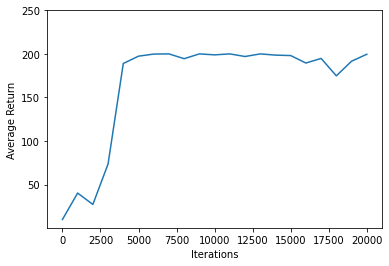
\includegraphics[width=0.5\textwidth]{Images/DQN20k.png}
\end{figure}
\begin{figure}[H]
\caption{Average return for Agent with 30,000 training iterations}
\centering
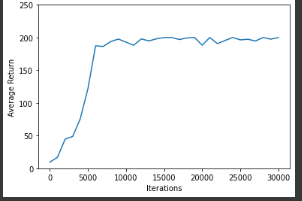
\includegraphics[width=0.5\textwidth]{Images/DQN30k.png}
\end{figure}
We can see from the figure above that the performance is not improving much after hitting 20k intervals. 
\begin{figure}[H]
\caption{Average return for Agent with 50,000 training iterations}
\centering
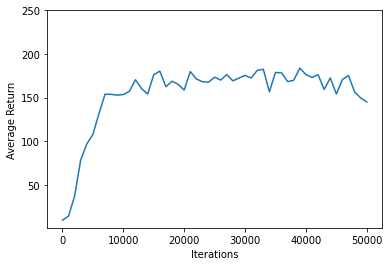
\includegraphics[width=0.5\textwidth]{Images/DQN50k.png}
\end{figure}
I also decided to see what effect training for 50k iterations would have, as we can see from the image below the performance actually decreases when after a certain number of iterations has been reached.  

\subsubsection{Actor Action Critique}

\subsection{Pros \& Cons}
\section{Conclusion}
\end{document}
